\subsection{Chaîne de transmission}

	\begin{defn}
		Un \textbf{canal de transmission est la donnée} est la donnée des probabilités $\{ Q(y \mid x), x \in \mathcal{X}, y \in \mathcal{Y} \}$.
	\end{defn}

	\begin{defn}
		La capacité d'information d'un canal est $C = \max_{p_X} I(X,Y)$ (maximisation sur les distributions de $X$), où $(X,Y) \sim p_x \cdot Q_{Y \mid X}$.
	\end{defn}

	\begin{pop}
		On a $0 \leq C \leq \min \{ \log (\abs{\mathcal{X}}), \log (\abs{\mathcal{Y}}) \}$.
	\end{pop}

	On a alors la \textbf{chaîne de transmission} suivante :
	\vspace{0.5em}

	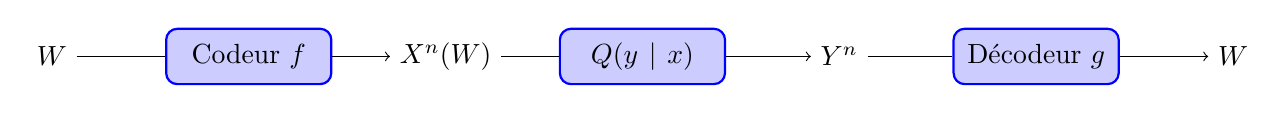
\begin{tikzpicture}
		\tikzstyle{block} = [rectangle, draw=blue, thick, fill=blue!20, text width=5.3em, text centered, rounded corners, minimum height=2em]
		\node (W) at (0,0) {$W$};
		\node [block] (f) at (2.5,0) {Codeur $f$};
		\node (X) at (5,0) {$X^n(W)$};
		\node [block] (Q) at (7.5,0) {$Q(y \mid x)$};
		\node (Y) at (10,0) {$Y^n$};
		\node [block] (g) at (12.5,0) {Décodeur $g$};
		\node (WT) at (15,0) {$\Hat{W}$};
		\draw (W) to (f);
		\draw [->] (f) to (X);
		\draw (X) to (Q);
		\draw [->] (Q) to (Y);
		\draw (Y) to (g);
		\draw [->] (g) to (WT);
	\end{tikzpicture}

	où $W$ et $\Tilde{W}$ sont des fonctions aléatoires à valeurs dans $\mathcal{M}$, l'ensemble des mots.
	$W$ est supposée suivre une loi uniforme.
	Pour un canal sans mémoire : $\proba(y^n \mid x^n(w)) = \prod_{i = 1}^n Q(y_i \mid x_i(w))$.
	Une \textbf{stratégie de transmission} désigne l'ensemble du codeur et du décodeur.

	Nos données sont $(M,n)$, avec $M = \abs{\mathcal{M}}$.

	\begin{defn}
		On note $R = \frac{\log_2 M}{n}$, en bits d'informations, le \textbf{taux de performance}.
	\end{defn}

	On veut maximiser $R$ tout en minimisant $P_e = \proba(\Tilde{W} \neq W) = \frac{1}{M} \sum_{w \in \mathcal{M}} \proba(g(Y^n) \neq w \mid X^n(w))$.

	\begin{defn}
		Un taux $R$ est dit \textbf{atteignable} s'il existe une suite de stratégies de codage $((M = 2^{nR},n))_{n \geq 1}$ telle que $P_e^{(n)} \overset{n \to +\infty}{\to} 0$.
	\end{defn}

	\begin{thm}
		Soit un canal $Q(y \mid x)$.
		On a :
		\begin{itemize}
			\item[\textbullet] $\forall R, R < C$, $R$ est atteignable,
			\item[\textbullet] $\forall R, R > C$, $R$ n'est pas atteignable.
		\end{itemize}
	\end{thm}

	\begin{note}
		Si $X,Y,Z$ forment une chaîne de Markov, on note $X - Y - Z$.
	\end{note}

	\begin{lem}
		Si $X - Y - Z$, $I(X;Y) \geq I(X;Z)$.
	\end{lem}

	\begin{lem}[\textbf{Inégalité de Fano}]
		Soit une chaîne $X - Y - \Hat{X}$.
		On a $1 + \proba(\Hat{X} \neq X) \cdot \log (\abs{\mathcal{X}}) \geq H(X \mid Y)$.
	\end{lem}

	\begin{lem}
		Soit $X^n$ et $Y^n$ l'entrée et la sortie d'un canal donné.
		Alors $I(X^n;Y^n) \leq nC$ avec $C$ la capacité du canal.
	\end{lem}


\subsection{Canal gaussien}

	Pour un canal gaussien on a $Y = X + Z$ avec $Z \sim \normale(0,\sigma^2)$ indépendant de $X$.
	
	Contrainte de puissance : le code $\{ x^n(m) \}_{m \in \mathcal{M}}$ doit satisfaire $\forall m \in \mathcal{M}, \frac{1}{n} \sum_{i = 1}^n x_i^n(w) \leq P$.
	
	\begin{thm}
		La capacité du canal gaussien $(P,\sigma^2)$ est $C = \max_{X, \esp(X^2) \leq P} I(X;Y) = \frac{1}{2} \log \left( 1 + \frac{P}{\sigma^2} \right)$ où $\frac{P}{\sigma^2}$ est le rapport signal sur bruit (SNR).
	\end{thm}


\subsection{Codage conjoint source - canal}

	Soit $S^n = S_1, S_2, \ldots, S_m$ une source i.i.d. d'alphabet $\mathcal{S}$.
	Puisque $\abs{A_\varepsilon^n} \doteq 2^{m H(S)}$ on a besoin de $m \cdot H(S)$ bits pour coder les séquences typiques, et l'on peut se restreindre à elles (compression sans erreur).
	Si l’on veut envoyer ensuite cette information à travers un canal de capacité $C$ il suffit que la longueur $n$ des mots code du codage de canal satisfasse $\frac{\log M}{n} = R \cdot H(S) < C$, où $R = \frac{m}{n}$.

	Lorsque l’on veut envoyer $S^n$ à travers un canal, on peut sans perte d’optimalié décomposer la procédure en 2 parties : comprimer $S^n$ (codage source) pour ensuite la protéger du bruit du canal en lui rajoutant de la redondance (codage de canal).


\subsection{Compression avec distorsion}

	\begin{defn}
		Une \textbf{fonction de distorsion} est de la forme
		$d \colon \begin{array}{ccc}
			\mathcal{X} \times \mathcal{X} & \to & \R_+ \\
			(x,\hat{x}) & \mapsto & d(x,\hat{x})
			\end{array}$.
	\end{defn}
	
	\begin{ex}
		\begin{itemize}
			\item[\textbullet] Distorsion de Hamming : $d(x,\hat{x})$ vaut $0$ si $\hat{x} = x$ et $1$ sinon.
			\item[\textbullet] Si $\mathcal{X} = \R$, $d(x,\hat{x}) = (x - \hat{x})^2$.
		\end{itemize}
	\end{ex}

	\begin{defn}
		La \textbf{distorsion} entre $x^n$ et $\hat{x}^n$ est donnée par $d(x^n,\hat{x}^n) = \frac{1}{n} \sum_{i = 1}^n d(x_i, \hat{x}_i)$.
	\end{defn}

	\begin{note}
		Fonction de codage : $f_n \colon \mathcal{X}^n \to \iniff{1}{2^{nR}}$.
		Fonction de décodage : $g_n \colon \iniff{1}{2^{nR}} \to \mathcal{X}^n$.
	\end{note}

	La distorsion associée à $(2^{nR},n)$ est $D = \esp \left[ d \left( X^n, g_n \circ f_n (X^n) \right) \right] = \sum_{x^n} p(x^n) d(x^n, g_n \circ f_n (x^n) )$.
	
	\begin{defn}
		$(R,D)$ est dit atteignable s'il existe $((2^{nR},n))_{n \geq 1}$ telle que $\limsup_{n \to \infty} \esp \left[ d \left( X^n, g_n \circ f_n (X^n) \right) \right] \leq D$.
		On note $R(D)$ le \textbf{taux atteignable minimal} avec distorsion $D$.
	\end{defn}

	\begin{thm}
		Pour $X$ donné, $R(D) = \min_{p_{\hat{x} \mid x}} I(X;\Hat{X})$.
	\end{thm}
	
	\begin{thm}
		Pour une source binaire i.i.d. de loi $\mathcal{B}(p)$ avec $p \leq \frac{1}{2}$ et une distorsion de Hamming, il vient\\
		$R(D) = \left\{ \begin{array}{ll}
			H_b(p) - H_b(D) & \text{si}\ 0 \leq D \leq p \\
			0 & \text{sinon}
			\end{array} \right. $.
	\end{thm}
